\documentclass{sig-alternate}

\usepackage[utf8]{inputenc}
\usepackage[T1]{fontenc}
\usepackage{graphicx}
\usepackage{amssymb}
\usepackage{amsmath}
\usepackage{mysymbols}
\usepackage{hyperref}
\usepackage{tikz}

\usepackage{xcolor}
\newcommand{\todo}[1]{\textcolor{red}{(#1)}}

\newcommand{\Cyc}{\Phi}  % Cyclotomic polynomial

\begin{document}

\title{Cool title to catch Lenstra's eye goes here}
\numberofauthors{3}
\author{
  \alignauthor Luca De Feo
  \alignauthor Javad Doliskani
  \alignauthor Éric Schost
}

\maketitle
\begin{abstract}
  We build towers.
\end{abstract}
\category{F.2.1}{Theory of computation}{Analysis of algorithms and problem complexity}[Computations in finite fields]
\category{G.4}{Mathematics of computing}{Mathematical software}
\terms{Algorithms,Theory}
\keywords{Finite fields, irreducible polynomials, extension towers, algebraic tori, elliptic curves.}

%%%

\section{Introduction}
\label{sec:intro}

Building arbitrary finite extensions of finite fields is a fundamental
task in any computer algebra system. Disregarding generic solutions
using multivariate algebra and Grobner bases, most systems are limited
to construct extensions of prime fields. There is one notable
exception: Magma~\cite{MAGMA} has implemented for a long time a
powerful system of ``compatibly embedded finite
fields''~\cite{bosma+cannon+steel97}, capable of building extensions
of any finite field and taking track of the embeddings between the
fields.

The system implemented in Magma, as described in the original paper,
uses linear algebra to describe the embeddings of finite fields. From
a complexity point of view this is far from optimal, indeed one may
hope to compute and apply the morphisms in (quasi)-linear time (in the
degree of the extension). Even worse, the quadratic memory
requirements make the system unsuitable for embeddings of large degree
extensions. Although the Magma core has evolved since the publication
of the paper, our experiments in Section~\ref{sec:bench} show that
embeddings of large extension fields are still out of reach in Magma.

In this paper we propose an approach based on polynomial arithmetic
rather than linear algebra, yielding much better performances. Our
solution only applies to some special cases, but we hope that it will
pave the way towards a complete solution. The technique we present is
similar to the one in~\cite{df+schost12} in that we construct families
of irreducible polynomials with special properties, then give
algorithms (called \emph{lift} and \emph{push}) that exploit the
special form of those polynomials to apply the embeddings. The
families of polynomials we use come from work of Lenstra and De Smit
on the algebraic closure of finite
fields~\cite{lenstra+desmit08-stdmodels}, and from work of Couveignes
and Lercier on constructing irreducible polynomials in quasi-linear
time~\cite{couveignes+lercier11}.

The focus of this paper is on the representation of extensions of
\emph{large} degree and their embeddings. We do not consider issues
related to special representations of small finite fields, such as
primitive polynomials, Zech logarithms, Conway polynomials, etc. A
user doing computations in a single, fixed, extension field will
clearly benefit more from these optimizations than from our
construction. However, a variety of computations in number theory and
algebraic geometry requires frequently constructing new extension
fields and moving elements from one to the other. Examples of these
algorithms are~\cite{df10} \todo{cite more}. Our construction makes
them feasible for much larger sizes than it was previously possible.

This paper is organized as follows. \todo{How?}

%%%

\section{Finite fields and embeddings}
\label{sec:finite-field-embedd}
We fix the following notation: $p$ is a prime, $d$ a positive integer,
$q=p^d$, $\F_p$ and $\F_q$ are the finite fields with $p$ and $q$
elements respectively. If $L/K$ is a field extension, we write
$\Tr_{L/K}$, $\Norm_{L/K}$ and $\Gal_{L/K}$ for the trace, the norm
and the Galois group of the extension, respectively. When the field
$L$ is clear from the context, we simply write $\Tr_K$ and $\Norm_K$,
and when the field $K$ is clear too, we may write $\Tr$ and $\Norm$.

The field $\F_q$ can be constructed as the splitting field of any
irreducible polynomial of degree $d$, we call this the \emph{defining
  polynomial} of $\F_q$. There are about $p^d/d$ such irreducible
polynomials over $\F_p$ \todo{cite something}, giving as many
different ways of representing $\F_q$. Furthermore, there is no
canonical way of establishing isomorphisms between them, indeed a
field with $p^d$ elements has $d$ automorphisms fixing $\F_p$.

A field with $p^d$ elements contains subfields with $p^n$ elements for
any $n|d$. For the same reasons as above, there is no canonical way of
embedding one finite field into another.

Let $\ell$ be another integer. We define the \emph{$\ell$-adic
  closure} of $\F_p$ as follows. Fix arbitrary embeddings
\begin{equation*}
  \F_p \subset \F_{p^\ell} \subset \F_{p^{\ell^2}} \subset \cdots,
\end{equation*}
the $\ell$-adic closure is the infinite field defined by
\begin{equation*}
  \F_p^{(\ell)} = \bigcup_{i>0}\F_{p^{\ell^i}}.
\end{equation*}
We also call an \emph{$\ell$-adic tower} the sequence of extensions
$\F_p,\F_{p^\ell},\dots$ When $\ell$ is prime, the Galois group of
$\F_p^{(\ell)}/\F_p$ is a procyclic group isomorphic to $\Z_\ell$, the
$\ell$-adic integers. Let $\bar{\F}_p$ be an algebraic closure of
$\F_p$, then there is a well known isomorphism
\begin{equation}
  \label{eq:tensor}
  \bar{\F}_p \isom \bigotimes_{\ell\text{ prime}} \F_p^{(\ell)},
\end{equation}
where the tensor products are over $\F_p$.

A \emph{root of unity} is an element of finite multiplicative order;
the element is said to be a \emph{$n$-th root} if its order divides
$n$, a \emph{primitive $n$-th root} if it is exactly $n$. Obviously,
every element of a finite field is a root of unity. The $n$-th
cyclotomic polynomial $\Cyc_n$ is the polynomial whose roots are the
primitive $n$-th roots of unity. It has integer coefficients and its
degree is $\euler(n)$. Viewed as a polynomial with coefficients in $\F_q$,
it splits into irreducible factors of degree equal to the order of $q$
in $\Z/n\Z$, and splits completely in an extension of the same
degree. We call this splitting field the $n$-th Kummer extension of
$\F_q$.

\paragraph{Algorithms}
Most computer algebra systems construct the field $\F_q$ by taking
degree $d$ polynomials at random until one irreducible is found. This
approach has a cost at least quadratic in the degree $d$. More
advanced constructions use Eq.~\eqref{eq:tensor}: they factor $d$ into
prime powers, for each prime power construct an extension of $\F_p$ of
that degree, then glue all the extensions together by taking
\emph{composita}.

The classical way of taking \emph{composita} is \todo{where?}

\begin{figure}
  \centering
  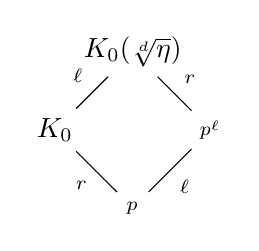
\begin{tikzpicture}[node distance=1.4cm]
    \node(Fp){$\F_p$};
    \node(K0)[above left of=Fp]{$K_0$};
    \node(K1)[above right of=K0]{$K_0(\sqrt[d]{\eta})$};
    \node(Fq)[above right of=Fp]{$\F_{p^\ell}$};
    \draw (Fp) edge node[auto]{\scriptsize$r$} (K0)
               edge node[auto,swap]{\scriptsize$\ell$} (Fq)
          (K1) edge node[auto,swap]{\scriptsize$\ell$} (K0)
               edge node[auto]{\scriptsize$r$} (Fq);
  \end{tikzpicture}
  \caption{Shoup's construction}
  \label{fig:shoup}
\end{figure}

Algorithms to construct extensions of degree a prime power can be
thought of as constructions for $\ell$-adic closures of
$\F_p$. Shoup's~\cite{shoup94} is summarized in
Figure~\ref{fig:shoup}. Let $\ell$ be a prime, the algorithm starts by
constructing $K_0$ the $\ell$-th Kummer extension of $\F_p$, then
looks for a non $\ell$-adic residue $\eta$ and uses it to construct a
degree $\ell$ extension $K_1$. This last step can be repeated several
times, to obtain an extension of degree $\ell^i$ of $K_0$. Finally it
takes the trace of a random element of $K_1$ down to $\F_{p^\ell}$ and
computes its minimal polynomial over $\F_p$, which is very likely to
be a defining polynomial for $\F_{p^\ell}$. Unless $K_0$ equals $F_p$,
Shoup's construction has quadratic complexity in $\ell$ \todo{Maybe
  this should be made more precise, with a discussion on modular
  composition}.  Couveignes and Lercier give an alternative
construction with complexity subquadratic in
$\ell$~\cite{couveignes+lercier11}; we will discuss it in
Section~\ref{sec:fibers}.


%%%

\section{Lenstra's and De Smit's tower}
\label{sec:LDtower}

Shoup's construction is non-deterministic, and it is shown that any
degree $\ell$ irreducible polynomial can be obtained that way. We now
describe a deterministic variant of Shoup's construction given by
Lenstra and De Smit~\cite{lenstra+desmit08-stdmodels}.

\begin{figure}
  \centering
  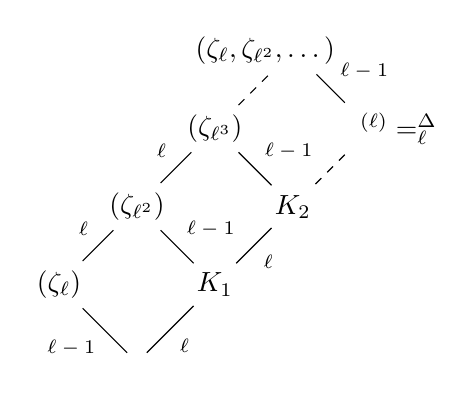
\begin{tikzpicture}[node distance=1.4cm]
    \node(Q){$\Q$};
    \node(Q0)[above left of=Q]{$\Q(\zeta_\ell)$};
    \node(K1)[above right of=Q]{$K_1$};
    \node(Q1)[above right of=Q0]{$\Q(\zeta_{\ell^2})$};
    \node(K2)[above right of=K1]{$K_2$};
    \node(Q2)[above right of=Q1]{$\Q(\zeta_{\ell^3})$};
    \node(Koo)[above right of=K2]{$\qquad \Q^{(\ell)} = \Q_\ell^\Delta$};
    \node(Qoo)[above right of=Q2]{$\Q(\zeta_\ell,\zeta_{\ell^2},\dots)\qquad$};
    \draw (Q) edge node[auto]{\scriptsize$\ell-1$} (Q0)
              edge node[auto,swap]{\scriptsize$\ell$} (K1)
          (K1) edge node[auto,swap]{\scriptsize$\ell-1$} (Q1)
               edge node[auto,swap]{\scriptsize$\ell$} (K2)
          (Q1) edge node[auto,swap]{\scriptsize$\ell$} (Q0)
          (Q2) edge node[auto]{\scriptsize$\ell-1$} (K2)
               edge node[auto,swap]{\scriptsize$\ell$} (Q1)
               edge[dashed] (Qoo)
          (Koo) edge[dashed] (K2)
               edge node[auto,swap]{\scriptsize$\ell-1$} (Qoo);
  \end{tikzpicture}
  \caption{The $\ell$-adic extension of $\Q$.}
  \label{fig:ladic}
\end{figure}

From now on, let $\ell$ be a prime different from the characteristic
$p$. For simplicity, we suppose $\ell\ne2$. Let $\zeta_{\ell^i}$ be
primitive $\ell^i$-th roots of unity, for algorithmic purposes we
further require that
$\zeta_{\ell^i}^\ell=\zeta_{\ell^{i-1}}$. Consider the tower of
extensions of the rationals given by
\begin{equation*}
  \Q \subset \Q(\zeta_\ell) \subset \Q(\zeta_{\ell^2}) \subset \cdots,
\end{equation*}
its limit is an infinite extension with Galois group isomorphic to
$\Z_\ell^\ast\isom\Delta\times\Z_\ell$, where $\Delta$ is the torsion
part of $\Z_\ell^\ast$, a cyclic group of order $\ell-1$. The
\emph{$\ell$-adic extension of $\Q$} is defined as the subfield fixed
by $\Delta$:
\begin{equation}
  \Q^{(\ell)} = \Q(\zeta_\ell, \zeta_{\ell^2}, \dots)^\Delta,
\end{equation}
it is the unique extension of the rationals having $\Z_\ell$ as Galois
group~\cite{lang1990cyclotomic,washington1997introduction}. The
construction of $\Q^{(\ell)}$ is summarized in
Figure~\ref{fig:ladic}. If we replace $\Q$ with a number field, we
obtain what is called the \emph{canonical $\ell$-adic extension}; its
Galois group is still $\Z_\ell$, but now there are others with this
property.

The cyclotomic extensions used to construct $\Q^{(\ell)}$ are
integral, thus it makes sense to reduce them modulo $p$. It turns out
that the reduction modulo $p$ of $\Q^{(\ell)}$ is an $\ell$-adic
closure of $\F_p$. Using number fields, this can be easily generalized
to build the $\ell$-adic closure of $\F_q$. We give two examples of
this construction.

\paragraph{$T_1$-type extensions}
Let $\ell$ be an integer (not necessarily prime) dividing $q-1$. In
this case the field $\F_q$ contains the primitive $\ell$-th roots of
unity and the map $x\mapsto x^{\ell}$ is not surjective on
$\F_q^\ast$. The construction is classical: select a non $\ell$-adic
residue $\zeta\in\F_q$ and construct $K_1,K_2,\dots$ as the tower of
extensions defined by the polynomials
\begin{equation}
  \label{eq:T1}
  \left|
  \begin{array}{rrrrr}
    X_{i+1}^\ell &- X_i\\
    &\vdots\\
    &&X_2^\ell &- X_1\\
              &&&X_1^\ell &- \zeta
  \end{array}
  \right.
\end{equation}
The only difference between Shoup's construction and Lenstra's and De
Smit's is the way $\zeta$ is selected. Shoup selects a random element
of $\F_q$ and tests it for non-residuosity, the test can be done in
$O(\log q)$ operations and an element is found after $O(1)$
trials. Lenstra and De Smit factor the $\ell$-th cyclotomic polynomial
to obtain a root $\zeta_0$, then take $\ell$-th roots until a non
$\ell$-adic residue is found. Compared to Shoup's algorithm this is
more expensive \todo{how much?}, but it has the benefit of being
deterministic if an arbitrary ordering is put on the $\ell$-th roots
of unity.

\paragraph{$T_2$-type extensions}
Let now $\ell$ be an odd \todo{isn't $\ell\ne2$ sufficient?} integer
(not necessarily prime) dividing $q+1$, this generalizes the way
Lenstra and De Smit handle $\ell=3$. The cyclotomic polynomial
$\Phi_\ell$ splits into $\euler(\ell)/2$ quadratic factors. Let $P$ be
one of these factors and let $\zeta_0$ be one of its roots (the choice
of $P$ can be made canonical by putting an ordering on the
factors). Then $\Norm(\zeta_0)=\zeta_0^{q+1}=1$ and
\begin{equation}
  \label{eq:quad-factor}
  P(X) = X^2 - X\Tr\zeta_0 + 1
\end{equation}
is the defining polynomial of $\F_q(\zeta_0)$. The cyclotomic tower (left
in Figure~\ref{fig:ladic}) is defined by the equations
\begin{equation}
  \label{eq:T2}
  \left|
  \begin{array}{rrrrr}
    \zeta_{i+1}^\ell &- \zeta_i\\
    &\vdots\\
    &&\zeta_2^\ell &- \zeta_1\\
              &&&\zeta_1^\ell &- \zeta_0\\
              &&&&P(\zeta_0)
  \end{array}
  \right.
\end{equation}
Its Galois group is isomorphic to $\Z/2\Z\times\Z_\ell$. 

At this point, Shoup's algorithm would select a random element of
$\F_q(\zeta_i)$ and take its trace down to a subfield of index
$2$. Following Lenstra and De Smit, we instead define some specific
Gauss periods generating the $\ell$-adic tower. These are the
following traces of the $\zeta_i$'s:
\begin{equation}
  \label{eq:T2-gauss-periods}
  \eta_i = \zeta_i + \zeta_i^{q^{\ell^i}} = \zeta_i + \zeta_i^{-1}.
\end{equation}
Then $\bigcup_i\F_q(\eta_i)$ is the $\ell$-adic closure of $\F_q$. By
Eq.~\eqref{eq:T2-gauss-periods}, the minimal polynomial of $\zeta_i$
over $\F_q(\eta_i)$ is $X^2 -\eta_iX+1$. By composition, it follows
that the minimal polynomial of $\zeta_i$ over $\F_q(\eta_{i-j})$ is
$X^{2\ell^j}-\eta_{i-j}X^{\ell^j}+1$. We deduce that the minimal
polynomial of $\eta_i$ over $\F_q(\eta_{i-j})$ is $Q_{i,j}$, where
\begin{equation}
  \label{eq:T2-relpols}
  Q_{i,j}(Y)^2 = \mathrm{Res}_X(X^{2\ell^j}-\eta_{i-j}X^{\ell^j}+1,\; X^2-YX+1).
\end{equation}
Indeed, by the well known properties of the resultant,
\begin{multline*}
  Q_{i,j}(Y)^2 = \prod_{\sigma\in\Gal_{\F_q(\zeta_i)/\F_q(\eta_{i-j})}}
  (\zeta_i^2 - Y\zeta_i + 1)^\sigma =\\
  % 
  \Norm_{\F_q(\eta_{i-j})}(\zeta_i) \prod_{\sigma\in\Gal_{\F_q(\zeta_i)/\F_q(\eta_{i-j})}} 
  (\zeta_i + \zeta_i^{-1} - Y)^\sigma =\\
  % 
  \left(\prod_{\sigma\in\Gal_{\F_q(\zeta_i)/\F_q(\eta_{i-j})}/\langle\tau\rangle}
    (\eta_i - Y)^\sigma\right)^2 =\\
  % 
  \left(\prod_{\sigma\in\Gal_{\F_q(\eta_i)/\F_q(\eta_{i-j})}}
    (\eta_i - Y)^\sigma\right)^2,
\end{multline*}
where the third equality is true because
$\Norm_{\F_q(\eta_{i-j})}(\zeta_i)=1$, as seen from the minimal
polynomial of $\zeta_i$, and where $\tau$ is the element of
$\Gal_{\F_q(\zeta_i)/\F_q(\eta_{i-j})}$ such that
$\tau:\zeta_i\mapsto\zeta_i^{-1}$.

As evident from the formula, the polynomials $Q_{i,j}$ depend on
$\eta_{i-j}$ and have the same form for any $i$. To explicitly compute
their general shape, we just need to compute
\begin{equation}
  Q_j(Y, z) = \sqrt{\mathrm{Res}_X(X^{2\ell^j}-zX^{\ell^j}+1, X^2-YX+1)}.
\end{equation}
Let $\zeta$ and $\zeta^{-1}$ be the two roots of $X^2-YX+1$, by direct
calculation we find
\begin{equation}
  Q_j = \zeta^{\ell^j} + \zeta^{-\ell^j} - z.
\end{equation}
The factor $p_{\ell^j}=\zeta^{\ell^j} + \zeta^{-\ell^j}$ is the $\ell^j$-th power sum
of $X^2-YX+1$, thus, using Newton's identities,
\begin{equation}
  \label{eq:simple}
  \begin{aligned}
    p_0 &= 2,\\
    p_1 &= Y,\\
    p_{\ell+1} &= Yp_{\ell} - p_{\ell-1}.
  \end{aligned}
\end{equation}
From Eq.~\eqref{eq:simple}, writing $p_\ell = \sum_i
c_{\ell,i}Y^{\ell-i}$, we obtain the relation
\begin{equation}
  c_{\ell,i} = c_{\ell-1,i} - c_{\ell-2,i-2}.
\end{equation}
We arrange these coefficients like in Pascal's triangle:
\begin{equation}
  \begin{tabular}{*{8}{c@{}}}
    &&&2\\
    &&1&&0\\
    &1&&0&&-2\\
    1&&0&&-3&&0
  \end{tabular}
\end{equation}
It is then evident that every second column is identically zero, and
that signs alternate in odd columns. We remove the zero columns and
take absolute values, i.e., we set $b_{n,k}=\lvert c_{n+k,2k}\rvert$, so
that the new coefficients satisfy the relation
\begin{equation}
  b_{n,k} = b_{n-1,k} + b_{n-1,k-1},
\end{equation}
which is the same as Pascal's relation. Indeed, we obtain the
$(1,2)$-Pascal triangle, also called Lucas' triangle~\cite{benjamin10}:
\begin{equation}
  \begin{tabular}{*{8}{c@{}}}
    &&&2\\
    &&1&&2\\
    &1&&3&&2\\
    1&&4&&5&&2
  \end{tabular}
\end{equation}
A special case of this fact was already proven by Gauss, and the
general proof is in~\cite[Proposition~1]{gurak06}.  It is well known
that the coefficients of Lucas' triangle are related to those of
Pascal's by
\begin{equation}
  \label{eq:lucas-tri}
  b_{n,k} = \binom{n}{k} + \binom{n-1}{k-1} = \frac{n+k}{n}\binom{n}{k}.
\end{equation}
One remarkable property of the Lucas triangle is that the
anti-diagonals sum up to the Lucas numbers:
\begin{equation}
  \sum_{k\ge0} b_{n-k,k} = \sum_{k\ge0} \lvert c_{n,2k}\rvert = L_n.
\end{equation}
A funny consequence of this property is the following equality on
complex numbers
\begin{equation}
  \label{eq:lucas-fun}
  p_\ell(i) = \sum_{k\ge0} c_{\ell,k}i^{\ell-k} = i^\ell L_\ell.
\end{equation}
By using Eq.~\eqref{eq:lucas-tri} and the sign alternation property,
we obtain 
\begin{gather}
  c_{\ell,2k} = (-1)^kb_{\ell-k,k} = (-1)^k\frac{\ell}{\ell-k}\binom{\ell-k}{k},\\
  \label{eq:lucas-recurrence}
  \frac{c_{\ell,2k+2}}{c_{\ell,2k}} = 
  -\frac{(\ell-2k)(\ell-2k-1)}{(\ell-k-1)(k+1)}.
\end{gather}
Eq.~\eqref{eq:lucas-recurrence} gives a formula to compute all the
coefficients of $Q_{i,j}$ using $O(\ell)$ operations. Of special
interest to us are the polynomials $Q_{i,i}$, defining each level of
the tower over the base field $\F_q$, and the polynomials $Q_{i,1}$,
defining each level over the previous one. We will come back to the
importance of these polynomials in Section~\ref{sec:lift-push}.


%%%

\section{Towers from irreducible fibers}
\label{sec:fibers}
Every tower obtained by the Lenstra-De Smit construction, as well as
many others, can be understood in a geometrical way using an intuition
of Couveignes and Lercier\cite{couveignes+lercier11}. Suppose we are
given algebraic groups $G/\F_q$, $G'/\F_q$ and a degree $\ell$ map
$\phi:G'\to G$ surjective over the algebraic closure. If $\phi$ is not
surjective over $\F_q$, then some points of $G'$ will have fibers
consisting of $\ell$ distinct points of $G$ living in an algebraic
extension of $\F_q$. If $\phi$ is chosen well enough, these fibers can
be made to be irreducible over $\F_q$, so that an annihilating
polynomial will be irreducible of degree $\ell$, as required. If the
construction can be repeated with a new map $\phi':G''\to G'$, and so
on, then one is able to construct a tower of extensions of degree
$\ell$, ultimately leading to an $\ell$-adic closure. We now show how
this idea applies to the two examples shown before, then how
Couveignes and Lercier apply it to elliptic curves.

\paragraph{Algebraic tori}
In the case where $\ell$ divides $q-1$, the algebraic group involved
is the multiplicative group $\mathbb{G}_m/\F_q$, and the map is the
$\ell$-th power map defined by $\phi:x\mapsto x^\ell$. Since the map
is an endomorphism of $\mathbb{G}_m$, it can be iterated, yielding
each of the $\ell^i$-th power maps. It is well known, then, that if
$\zeta$ is a non $\ell$-adic residue, the polynomials
$X^{\ell^i}-\zeta$ corresponding to the fibers of $\phi^i$ are
irreducible over $\F_q$.

The case where $\ell$ divides $q+1$ is more interesting. Now
$\F_q(\zeta_i)$ is a quadratic extension of $\F_q(\eta_i)$. The
multiplicative subgroup defined by
\begin{equation}
  \label{eq:T2-def}
  T_2 = \{\alpha\in\F_q(\zeta_i) \;|\; \Norm_{\F_q(\eta_i)}(\alpha) = 1\}
\end{equation}
is called the \emph{maximal torus} of $\F_q(\zeta_i)$. Seen as an
algebraic group defined over $\F_q$, it has dimension one, cardinality
$q+1$, and is isomorphic to $\mathbb{G}_m$ over the algebraic closure.

We now write down explicit algebraic equations for $T_2/\F_q$ and its
$\ell$-th power map, we suppose for simplicity that the characteristic
of $\F_q$ is different from $2$. Let $\sigma$ be the non trivial
element of the Galois group of $\F_q(\zeta_i)/\F_q(\eta_i)$, so that
$\sigma(\zeta_i)=\zeta_i^{-1}$. Set $\theta = \zeta_i -
\sigma(\zeta_i)$, then $\sigma(\theta)=-\theta$ and $\theta^2 =
\eta_i^2-4$, so that
\begin{equation}
  \F_q(\zeta_i) = \F_q(\theta) = \F_q\left(\sqrt{\eta_i^2-4}\right).
\end{equation}
Because of our assumption on the characteristic, $(1/2, \theta)$ is a
basis of $\F_q(\zeta_i)$ seen as a vector space over
$\F_q(\eta_i)$. Hence, every element $\alpha\in\F_q(\zeta_i)$ can be
uniquely written as $x/2 + y\theta$ with $x,y\in\F_q(\eta_i)$. By
virtue of Eq.~\eqref{eq:T2-def}, an element $\alpha=x/2+y\theta$
belongs to $T_2$ if and only if
\begin{equation}
  \label{eq:Pell}
  \Norm\left(\frac{x}{2} + y\theta\right) = 
  \left(\frac{x}{2} + y\theta\right)\left(\frac{x}{2} - y\theta\right) =
  \frac{x^2}{4} - \theta^2y^2 = 1.
\end{equation}
Eq.~\eqref{eq:Pell} defines a conic section over $\F_q(\eta_i)$, known
as \emph{Pell conic}. It has a group law induced by multiplication in
$T_2$: its neutral element is $(2,0)$, and it is easily checked that
the addition of two points is defined by
\begin{equation}
  \label{eq:Pell-add}
  (x,y)\oplus(x',y') =
  \left(\frac{xx'}{2} + 2\theta^2yy', \frac{xy' + x'y}{2}\right).
\end{equation}
We denote by $[\ell](x,y)$ the $\ell$-th scalar multiple of the point
$(x,y)$ on the Pell conic. Thanks to Eq.~\eqref{eq:Pell-add}, we
verify that
\begin{equation}
  \label{eq:Pell-rec}
  [\ell](x,y) = \bigr(p_\ell(x), yq_\ell(x)\bigl),
\end{equation}
where $p_\ell$ is defined as in Eq.~\eqref{eq:simple}, and $q_\ell$ is
defined by
\begin{equation}
  \label{eq:fibonacci}
  \begin{aligned}
    q_0 &= 0,\\
    q_1 &= 1,\\
    q_{\ell+1} &= Yq_{\ell} - q_{\ell-1} = p_\ell + q_{\ell-1}.
  \end{aligned}
\end{equation}
In particular, the coefficients of $q_\ell$ correspond to the
anti-diagonals of Pascal's triangle with alternating signs, and we
have the analogue of Eq.~\eqref{eq:lucas-fun}:
\begin{equation}
  \label{eq:fibonacci-fun}
  q_{\ell+1}(i) = \sum_{k=0}^{\lfloor\ell/2\rfloor} p_{\ell-2k}(i) = 
  i^\ell F_{\ell+1},
\end{equation}
where $F_\ell$ is the $\ell$-th Fibonacci
number. Eq.~\eqref{eq:Pell-rec} is proved by induction, indeed it is
easily checked that $[0](x,y) = (2,0)$ and $[1](x,y)=(x,y)$, and the
general case follows from \todo{This can be safely removed}
\begin{multline}
  [\ell+1](x,y) = \bigl(p_\ell(x), yq_\ell(x)\bigr) \oplus (x,y) =\\
  \left(\frac{xp_\ell(x)}{2} + 2\theta^2y^2q_\ell(x),
    y\frac{p_{\ell}(x) + xq_\ell(x)}{2}\right) =\\
  \left(x\frac{p_\ell(x) + xq_\ell(x)}{2} - 2q_\ell(x),
    y\frac{p_{\ell}(x) + xq_\ell(x)}{2}\right) =\\
  \bigl(xq_{\ell+1}(x) - 2q_\ell(x), yq_{\ell+1}(x)\bigr) = 
  \bigl(p_{\ell+1}(x), yq_{\ell+1}(x)\bigr).
\end{multline}

Now, if $(\eta,\eta')$ is a point on the Pell conic of order different
from $2$, its fiber via the map $[\ell]$ is composed of $\ell$ points
with distinct abscissas, and the polynomial $p_\ell-\eta$ vanishes on
each of them with multiplicity one. In particular $\zeta_i =
\eta_i/2+\theta/2$, and we have already shown that $p_\ell-\eta_i$ is
irreducible over $\F_q(\eta_i)$, and is in fact the minimal polynomial
of $\eta_{i+1}$.  By iterating the map $[\ell]$, we obtain the same
family of irreducible polynomials
\begin{equation}
  Q_{i,j}(Y) = p_{\ell^j}-\eta_{i-j}
\end{equation}
from the previous Section.

We obtain an interesting insight from this geometric
interpretation. In the case where $\ell$ divides $q-1$ we had the
choice between selecting a specific root of unity, or picking any
random $\ell$-adic non-residue to initialize the family of irreducible
polynomials. In the same fashion, $\eta_0$ is not the only possible
starting point: we can pick any point $(\eta,\eta')$ corresponding to
an $\ell$-adic non-residue of $T_2$, and its fiber will necessarily be
irreducible. Algorithmically, in the first case we would factor the
cyclotomic polynomial \todo{how much does it cost?}, while in the
second case we would take random points on the conic and test their
order using $O(\log q)$ operations in $\F_q$.

The two previous cases involving the tori $T_1$ and $T_2$ are very
special ones. In general, if $n$ is the order of $q$ modulo $\ell$, we
define the \emph{maximal torus} of $\F_{q^n}$ as
\begin{equation}
  \label{eq:T2-def}
  T_n = \{\alpha\in\F_{q^n} \;|\; \Norm_{\F_{q^m}}(\alpha) = 1 
  \text{ for any $m|n$} \}.
\end{equation}
This is an algebraic group over $\F_q$ of dimension $\euler(n)$ and
cardinality $\Phi_n(q)$, isomorphic to $\mathbb{G}_m^{\euler(n)}$ over
the algebraic closure. Compared with the previous cases, we are faced
with two problems. First, multiplication by $\ell$ is now a degree
$\ell^{\euler(n)}$ map, thus its fibers have too many points and are
not irreducible in general. Second, it is an open question whether
$T_n$ can be parameterized using $\euler(n)$
coordinates~\cite{rubin-silverberg+crypto03,rubin+silverberg03,voskresenskii98};
but even assuming it can be, we are still faced with the problem that
the fibers of algebraic maps would be described as zero-dimensional
objects embedded in a $\euler(n)$-dimensional space. Going from such a
description to an irreducible univariate polynomial is not a trivial
task algorithmically.

\paragraph{Elliptic curves}
Since it seems hard to deal with higher dimensional algebraic tori, it
makes sense to look at other algebraic groups. Being one-dimensional,
elliptic curves are good candidates. We quickly review Couveignes' and
Lercier's construction and refer to~\cite{couveignes+lercier11} for
details.

Let $\ell$ be a prime different from $p$ and not dividing $q-1$. Let
$E_0$ be an elliptic curve whose cardinality is a multiple of
$\ell$. By Hasse's bound, this is only possible if $\ell\le q +
2\sqrt{q} + 1$. An \emph{isogeny} is an algebraic group morphism
between two elliptic curves that is surjective in the algebraic
closure; it is said to be rational over $\F_q$ if it is invariant
under the $q$-th power map. A rational isogeny between two curves
exists if and only if they have the same number of points over
$\F_q$. The degree of an isogeny is its degree as an algebraic map; an
isogeny is separable if and only if its degree is prime to $p$, in
which case its kernel contains as many points as the degree. A
connected component of the graph whose vertices are elliptic curves up
to isomorphism and whose edges are rational isogenies of degree $\ell$
is called an \emph{$\ell$-isogeny
  volcano}~\cite{kohel,fouquet+morain02}. It is an undirected graph
and in the specific case at hand it is a
cycle. Figure~\ref{fig:volcano} shows an example of volcano containing
$E_0$; from now on, we denote by $E_0,E_1,\dots$ the curves in the
same volcano as $E_0$, the order of the labeling will be precised in
the next paragraphs.

\begin{figure}
  \centering
  \begin{tikzpicture}
  \end{tikzpicture}
  \caption{The $\ell$-isogeny volcano}
  \label{fig:volcano}
\end{figure}

Suppose that $p\ne2,3$ and let $E_0$ be expressed as the locus
\begin{equation}
  E_0 \;:\; y^2 = x^3 + ax + b,
  \quad\text{with $a,b\in\F_q$},
\end{equation}
plus one point at infinity.  Let $H\subset E_0$ be a finite subgroup of
$E_0$.  Vélu's formulas~\cite{velu71} express the isogeny $\phi$ whose
kernel is $H$ as a rational fraction
\begin{equation}
  \begin{aligned}
    \phi: E_0 &\to E',\\
    (x,y) &\mapsto \left(\frac{f(x)}{g(x)}, y\left(\frac{f(x)}{g(x)}\right)'\right).
  \end{aligned}
\end{equation}
Let $\ell$ be the cardinality of $H$, then $g$ is a square polynomial
of degree $\ell-1$ vanishing on the abscissas of the points of $H$,
while $f$ is a polynomial of degree $\ell$. Algorithmically, Vélu
isogenies can be computed using $O(\Mult(\ell))$ operations in $\F_q$.

Under the former assumptions on $\ell$, the $\ell$-Sylow subgroups of
each of the $E_i$'s are isomorphic to $\Z/\ell^e\Z$ for some
$e\ge1$. For each $E_i$ we consider the unique subgroup $H_i$ of order
$\ell$ and we construct the Vélu isogeny $\phi_i:E_i\to E_{i+1}$. For
an arbitrary $i$, let $P$ be a point on $E_{i+1}$ of order divisible
by $\ell^e$, Couveignes and Lercier show that its fiber by $\phi_i$ is
irreducible of cardinality $\ell$. Hence, if the order of $P$ is not
$2$, and if $\eta$ is the abscissa of $P$, the polynomial
\begin{equation}
  \label{eq:isog-fiber}
  f_i(x) - \eta g_i(x)
\end{equation}
is irreducible of degree $\ell$.

%%%

\section{Lifting and pushing}
\label{sec:lift-push}

The two algorithms given in the notes for the rational fraction case
(and how they reduce to the polynomial case).

%%%

\section{The general case}
\label{sec:general}

Composita, general LD-towers, other algebraic tori, higher dimensional
fibers...

%%%

\section{Benchmarks}
\label{sec:bench}

Sage implementation and timings.

%%%

\section{Aknowledgements}
De Feo would like to thank Antoine Joux.

\bibliographystyle{abbrv}
\bibliography{defeo}
\end{document}


% Local Variables:
% mode:flyspell
% ispell-local-dictionary:"american"
% mode:TeX-PDF
% mode:reftex
% End:
%
% LocalWords:  Isogeny abelian isogenies hyperelliptic supersingular Frobenius
% LocalWords:  isogenous embeddings Vélu

